\documentclass[a4paper,12pt]{article}
\usepackage[utf8]{inputenc}
\usepackage{authblk}
\usepackage{amssymb}
\usepackage{amsmath}
\usepackage{amsfonts} % for mathbb{1} indicator
\usepackage{listings}
\usepackage{xcolor}
\usepackage{pgf-pie} % for pie chart

\definecolor{codegreen}{rgb}{0,0.6,0}
\definecolor{codegray}{rgb}{0.5,0.5,0.5}
\definecolor{codepurple}{rgb}{0.58,0,0.82}
\definecolor{backcolour}{rgb}{0.95,0.95,0.92}

\lstdefinestyle{mystyle}{
    backgroundcolor=\color{backcolour},
    commentstyle=\color{codegreen},
    keywordstyle=\color{magenta},
    numberstyle=\tiny\color{codegray},
    stringstyle=\color{codepurple},
    basicstyle=\ttfamily\footnotesize,
    breakatwhitespace=false,
    breaklines=true,
    captionpos=b,
    keepspaces=true,
    numbers=left,
    numbersep=5pt,
    showspaces=false,
    showstringspaces=false,
    showtabs=false,
    tabsize=2
}

\lstset{style=mystyle}

\providecommand{\keywords}[1]{\textbf{Keywords: } #1}

%opening
\title{BTMX Technical Report}

\author{The BITMarkets team}

\begin{document}

\maketitle

\begin{abstract}

We present you the technical report of BTMX, an ERC20 token that resides on the Polygon blockchain that will enable
the users of the BITMarkets platform to perform cryptocurrency exchanges with low fees,
to participate in initial coin offerings and exchange offerings and to
vote on the ecological and social impact investments of the company.

\end{abstract}

\keywords{bitmarkets, blockchain, ico, polygon, solidity}

\section{Introduction}

Digital tokens provide individuals and organizations with a robust, decentralized
method of exchanging value while using a familiar accounting unit.
Blockchains are cryptographically secured global ledgers of transactions that can be
audited by the public.
Smart contracts are computational logic that can be tied to a digital token in order to
augment its basic functionality with various mechanisms such as automated market marking, transaction fees, locking mechanisms,
without the ability of a central authority to block their execution.
This can add an economic layer to digital or physical activities
that were not even conceivable 12 years ago.

An ERC20 token uses the peer-to-peer network of an existing blockchain that is compatible
with the so-called Ethereum Virtual Machine (EVM) to operate with
no central authority or banks.
Managing transactions and the issuing of tokens is carried out by the network of the
blockchain's nodes, or servers, following the instructions outlined by the token's
accompanying smart contract.
We believe that the Polygon blockchain is the most suitable home for our token
because it builds on the already proven technology of Ethereum while improving on the
transaction costs and speed.

Tokens can be bought through online trading platforms with traditional currencies or
other cryptocurrencies,
through smart contracts running on the blockchain in exchange for the native
cryptocurrency of the blockchain or another token, or in personal transactions where the
sender and recipient agree on an exchange rate in person.
The token trading process itself is identical to the typical trading process.

In our exchange platform, trading pairs that involve BTMX will have lower exchange fees
than those that don't.
Moreover, users that hold more than 20\% of their portfolio value in BTMX
will be eligible for airdrops, NFT lotteries and other perks that will be announced in the future.
Finally, holders of BTMX will be able to participate in platform exclusive ICOs and IEOs,
which will be a great way for investors to invest in vetted, high impact projects that
they may find interesting.


\section{Token}

Digital tokens are stored in ``addresses'' on the blockchain network and
their owners can send them to other users in the network by issuing transactions signed by
their private key.
A private key is essentially a random number between $1$ and $2^{256}$,
converted to 64 hexadecimal digit representation,
while the public key is a set of coordinates $(x,y)$ calculated from the private key on the
$\text{secp}256\text{k}1$ curve $y^2 = x^3 + 7$ over the finite field
$\mathbb{Z}_{2^{256}-2^{32}-977}$.
The magic of a blockchain ``account opening'' is that the private key can be generated offline and
it will produce a perfectly valid destination address for a cryptocurrency transaction.
This is contrary to opening a bank account where the procedure takes days, requires
extensive KYC checks and the eventual account is controlled by a bank which can
effectively close it or freeze at any given time.
In the example of Ethereum, and consequently Polygon,
``wallet'' address is the last 20 bytes of the Keccak256 hash of the public key.
If someone knows a private key, they can trivially calculate their corresponding public key
and their wallet address, but someone who knows only the address or the public key cannot
reproduce the private key from it. Without the private key, a user cannot sign transactions.

\subsection{ERC20}
For out token, we will use the ERC20 token standard, which is a standard for fungible
tokens where each unit is equal in value and type to any other unit of the same token.
In this standard, the smart contract that governs the
token needs to implement a set of specific publicly accessible functions that
allow external programs to interact with the token.
The first set of functions has to do with the characteristics of the token, such as its name, its symbol, the number of decimals that it has and the total supply of tokens in existence:

\begin{lstlisting}[language=C++, caption=ERC20 Solidity qualitative function signatures.]
function name() public view returns (string);
function symbol() public view returns (string);
function decimals() public view returns (uint8);
function totalSupply() public view returns (uint256);
\end{lstlisting}
The rest of the functions in the ERC20 standard have to do with getting the balance of
an address,
the issuing of a transfer from one address to the other,
the so-called ``approval'', which is an operation that allows one address to delegate
the spending of some amount of its balance to another address, and the getter of the total allowance that this second address is approved to spend:

\begin{lstlisting}[language=C++, caption=ERC20 Solidity operational function signatures.]
function balanceOf(address) public view returns (uint256);
function transfer(address to, uint256) public returns (bool);
function transferFrom(
    address from,
    address to,
    uint256 amount
) public returns (bool);

function approve(address to, uint256) public returns (bool)
function allowance(
    address owner,
    address spender
) public view returns (uint256);
\end{lstlisting}
A smart contract that adheres to the ERC20 standard also emits two events, namely a successful transfer and a successful approval:
\begin{lstlisting}[language=C++, caption=ERC20 Solidity events.]
event Transfer(
    address indexed from,
    address indexed to,
    uint256 value
);

event Approval(
    address indexed owner,
    address indexed spender,
    uint256 value
);
\end{lstlisting}

\subsection{Extensions}
Other than the basic functionality of an ERC20-compliant smart contract, we have authored
some extensions that adhere to our own business model and will help us enforce our code of conduct
regarding the use of our products and services.

\subsubsection{Fees}

At the time of the deployment of the main token smart contract on the blockchain,
an extension that handles the fees from every token transfer is also deployed.
This extension calculates the transfer fees that will be distributed to two company-controlled wallets, based on prespecified percentages on the total amount of a transfer that are made available on deployment. These fees are removed from the transfer amount.

The two wallets that will receive the fees are an \textit{ESG fund} and a \textit{company rewards} wallet. The fees will be 0.1\% each and they will apply to all transfers above 1000 tokens.

We have also added the functionality to exclude some addresses from fee collection, because their ability to transact freely is instrumental to our smart contract functionality.
The three wallets that are excluded from fee collection automatically are the company liquidity wallet, the company rewards wallet and the ESG fund. We also set a separate wallet as an admin of the feeless list on deployment, and we set a limit of 4 addresses that can transact freely with our token.
The feeless functionality can be accessed publically by the following methods:

\begin{lstlisting}[language=C++, caption=Solidity feeless functions.]
function addFeeless(address) public virtual;
function removeFeeless(address) public virtual;
function isFeeless(address) public virtual returns (bool);
\end{lstlisting}
The corresponding events that are emitted on successful completion of the state-mutating functions are:
\begin{lstlisting}[language=C++, caption=Solidity feeless events.]
event FeelessAdded(address indexed);
event FeelessRemoved(address indexed);
\end{lstlisting}

\subsubsection{Blacklisting}

The other token-related smart contract that will be deployed is one with blacklisting functionality, meaning that if an address is on this list, it will not be able to transact with our token. The wallet that will be the admin of the blacklist is a company-controlled one.
The methods that are exposed by this contract are the following:

\begin{lstlisting}[language=C++, caption=Solidity blacklist functions.]
function addBlacklisted(address) public virtual;
function removeBlacklisted(address) public virtual;
function isBlacklistAdmin(address) public virtual
    returns (bool);
function isBlacklisted(address) public virtual
    returns (bool);
\end{lstlisting}
The events that are emitted from the mutating functions are:

\begin{lstlisting}[language=C++, caption=Solidity blacklist events.]
event BlacklistedAdded(address indexed);
event BlacklistedRemoved(address indexed);
\end{lstlisting}

\section{Distribution
}
For BTMX, the total minted supply will be $300\text{ }000\text{ }000$ tokens,
which will be divided into three equal parts.
The first $100\text{ }000\text{ }000$ tokens will be sold in public and private sales for fundraising.
The second $100\text{ }000\text{ }000$ will be allocated to the wallets of the
BITMarkets team and to wallets for special activities such as
conferences, marketing campaigns, airdrops etc. and our partners.
The rest of the tokens will be held by a company wallet
that will be used as a liquidity vault which will periodically ``burn'' some portion of its tokens in order to diminish the token supply to the eventual point of $200\text{ }000\text{ }000$ final supply.
This last wallet's private key will not be owned by one single entity, but rather it will
be split in at least 9 Shamir shares, which will be distributed to members of the developer team and
external partners and it will only be possible to recreate it if at least 5 of them coordinate with each other.
This wallet will be the minting wallet, therefore it will also hold the sales funds and it will provide allowance of
$100\text{ }000\text{ }000$ tokens to the smart contracts that will govern the crowdsales.

\begin{center}
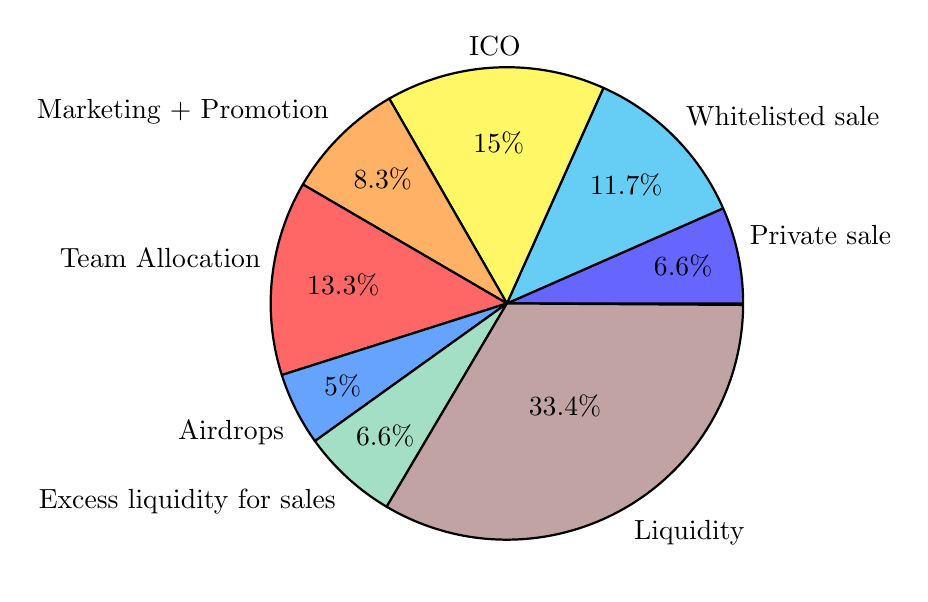
\begin{tikzpicture}
\pie{6.6/Private sale,
11.7/Whitelisted sale,
15/ICO,
8.3/Marketing + Promotion,
13.3/Team Allocation,
5/Airdrops,
6.6/Excess liquidity for sales,
33.4/Liquidity}
\end{tikzpicture}
\end{center}

\section{Crowdsales}

One third of the initial supply of BTMX will be sold in public and private sales. The smart contracts that govern these sales will have a combined allowance
of $100\text{ }000\text{ }000$ tokens from the company wallet to distribute to the buyers.
The smart contracts expect to trade MATIC,
Polygon's native cryptocurrency, with BTMX.
The company's Ethereum wallet will receive the MATIC that the buyer sends to the crowdsale
smart contracts and the contract will send them in return the amount of BTMX that
corresponds to the rate that is derived from the contract's code. The BTMX comes from the company-controlled liquidity wallet,
provided that it does not exceed the contract's allowance. The most important publicly-exposed methods of public and private crowdsale contracts are the following:
\begin{lstlisting}[language=C++, caption=Solidity common crowdsale function signatures]
function buyTokens(address buyer) public payable;
function getContribution(address buyer) public view returns (uint256);
function remainingTokens() public view returns (uint256);
function token() public view returns (IERC20);
function tokenWallet() public view returns (address);
function wallet() public view returns (address payable);
function weiRaised() public view returns (uint256);
\end{lstlisting}

Every sale will happen in a limited time window that will be specified on deployment.
In order for external programs to track their timing, the smart contracts provide the following functions:
\begin{lstlisting}[language=C++, caption=Solidity crowdsale timing function signatures]
function isOpen() public view returns (bool);
function hasClosed() public view returns (bool);
 (uint256);
function paused() public returns (bool);
function openingTime() public view returns
function closingTime() public view returns (uint256);
\end{lstlisting}

The smart contracts have algorithmic safeguards in order to ensure fair access to
the sales for as many buyers as possible.
The first and most obvious safeguard is that the hard cap of the sale will be
$100\text{ }000\text{ }000$ tokens. Two publicly accessible methods that give feedback regarding these safeguards are:
\begin{lstlisting}[language=C++, caption=Solidity public crowdsale cap function signatures.]
function cap() public view returns (uint256);
function capReached() public view returns (bool);
\end{lstlisting}
The second safeguard is that an individual address will have
both a tariff to participate and an individual cap to contribute:
\begin{lstlisting}[language=C++, caption=Solidity public crowdsale tariff/cap function signatures.]
function getInvestorCap() public view returns (uint256);
function getInvestorTariff() public view returns (uint256);
function investorCap() public returns (uint256);
function investorTariff() public returns (uint256);
\end{lstlisting}
The tariff will be at least $100$ MATIC and the cap will be at most $20000$ MATIC.
The timing of the sale is also written in code so no buyer can exchange MATIC for BTMX
with the conditions that we discussed at a time prior to the specified opening and after the closing time.

The contract will emit the following event on successful purchase:
\begin{lstlisting}[language=C++, caption=BTMX ICO events.]
event TokensPurchased(
  address indexed purchaser,
  address indexed beneficiary,
  uint256 value,
  uint256 amount
);
\end{lstlisting}

Users who are not in possession of a decentralized Ethereum, Polygon wallet will be able to
participate in the crowdsales by exchanging their traditional currency to BTMX
on the BITMarkets platform. They will need to pass a basic KYC check in order to exchange
``fiat'' for MATIC and then we will deposit their MATIC into the company wallet, which
will then trigger a server-side transfer of the corresponding to the predefined individual
exchange rate BTMX tokens to the client's platform-managed Polygon wallet.

\subsection{Whitelisted sales}

There will be both a private and a public whitelisted crowdsales that will happen before the ICO.
In the case of the private crowdsale, the whitelist will be prespecified.
In the case of the public whitelisted crowdsale, the company will provide a way for prospective buyers to make it into the whitelist by completing a number of tasks that will promote the company.
The publicly accessible functions that are relevant to the whitelist are the following:

\begin{lstlisting}[language=C++, caption=Solidity whitelisted crowdsale function signatures.]
function addWhitelisted(address) public virtual;
function removeWhitelisted(address) public virtual;
function isWhitelistAdmin(address) public view returns (bool)
function isWhitelisted(address) public view returns (bool);
\end{lstlisting}

The contracts will emit the following events on successful whitelisting and dewhitelisting:
\begin{lstlisting}[language=C++, caption=Solidity crowdsale whitelist events.]
event WhitelistedAdded(address indexed account);
event WhitelistedRemoved(address indexed account);
\end{lstlisting}

\subsection{ICO}
In the public crowdsale, the rate of MATIC over BTMX will decrease overtime,
meaning that the initial rate of exchange will be higher than the final one, and this
decrease will happen in a linear manner overtime.
This means that an early buyer will have to
deposit less MATIC for a bigger amount of BTMX compared to a late one.
The initial rate will be
$100$ BTMX for $1$ MATIC and it will linearly reduce to $10$ BTMX for $1$ MATIC.
The publicly accessible methods of the public crowdsale contracts regarding the trading rate are:
\begin{lstlisting}[language=C++, caption=Solidity public crowdsale rate function signatures.]
function initialRate() public view returns (uint256);
function finalRate() public view returns (uint256);
function getCurrentRate() public view returns (uint256);
\end{lstlisting}
This is in contrast to the private whitelisted crowdsales where we will use a prespecified, invariant trading rate.

\section{Vesting}

In order to ensure fair use of BTMX by the team and to reduce the volatility of its exchange price in the short run, there is a locking and vesting functionality built into the crowdsales and the team allocation contracts.

The vesting will occur linearly and will start from a point in time that is called the ``cliff''.
As time goes by, more and more tokens are unlocked from the purpose-generated locking wallets and are claimable by their original owners.
The functions that expose this functionality to the public are the following:

\begin{lstlisting}[language=C++, caption=Solidity vesting function signatures.]
function vestingWallet(address beneficiary) public view returns (address);
function vestedAmount(address beneficiary) public view returns (uint256);
function withdrawTokens() public;
\end{lstlisting}

In the crowdsale contracts, the vesting functionality intercepts the transfer of BTXM to the beneficiary, generates a vesting wallet with the cliff and vesting duration that corresponds to each sale and transfers the purchased BTMX token to that wallet.
The mapping of the beneficiary and their vesting wallet is stored on the blockchain and it is visible to everyone.

In the case of the team allocation, there will exist a special smart contract that will be deployed along with the BTMX token contract, which will have a ``whitelist'' of the team members' Ethereum wallets, an allowance that equals the team allocation amount from the company minting wallet and a list that corresponds to each team member's percentage. The members will be able to call a special ``participate'' function which will automatically send their tokens to a vesting wallet with a cliff of 6 months and a duration of 3 years.

\section{Utility}

Holders of BTMX will enjoy exclusive perks on our platform and on the blockchain.
We will periodically release exclusive airdrops, NFT lotteries when we start introducing
collections in our platform, reduced exchange fees for trading pairs that include BTMX
and many more.

The most interesting use case will come in Q1 of 2023 where we will introduce an ICO
platform where promising projects with little-to-no marketing budget will be able to list
their upcoming offerings on it and exchange a predefined amount of their tokens with BTMX.
BTMX investors will be able to participate in these sales inside our platform and our
contract logic will handle the transfer of their newly purchased tokens to their wallets.
Our platform will provide this service to the chosen projects in exchange for 10\% of their
accumulated funds.
We will also put 2 out of every 5 slots in the list of upcoming ICOs into hourly auctions
in order to cover the cost of marketing for all the projects and to monetize the benefit
of high placement advertising.

We will also create utility from the transaction costs of BTMX. Specifically,
0.5\% of the transferred amount from one address to another will go to
a specially designated wallet that will serve as the social investment arm of our
operation.
Our goal is for the BTMX holders to be able to participate in Governance votes that
will determine the purpose of the accumulated ``social investment'' units every 6 months.
The BITMarkets team will put together a list of all the potential investment targets and
the community of investors will hold a vote on the blockchain that determines the top 5
projects that will receive the funds and a corresponding smart contract will execute the
transactions.

\section{Conclusion}

This was the technical analysis of BTMX, an ERC20 token that will reside on the Polygon
blockchain. It's a token whose utility will have ramification in both the digital and
the physical world. Our BITMarkets platform will be more that an exchange platform and
BTMX will be the native currency to its ecosystem. Projects with great potential will
benefit from the vibrant investor community that we will host and developer teams that
focus on the technical aspect of their innovation will be able to offload the burden of
marketing, ICO design and investor search to us.
It is our hope that this will make BITMarkets the go-to place for bright innovators and
socially-conscious investors alike.

\end{document}
